\documentclass{spisok-article}

\title{Название статьи\thanks{ По сноске может быть информация о том,
    кем и чем поддержана работа. Если никем и ничем, то сноску нужно
    убрать.  Сноски вставляются в конец страницы стандартными
    средствами.}
}

\author{Список авторов с электронными адресами, должностями/учебными
  статусами и организациями, например:\\
  Луцив Д. В.,
  ст. преп. кафедры системного программирования СПбГУ,
  dluciv@math.spbu.ru\thanks{Если грантополучателей требуется указать
  лично --- тоже никаких препятствий.}
}

\begin{document}

\maketitle

\begin{abstract}
СПИСОК (Системное Программирование, Информационные Системы,
Обеспечение Качества) --- периодическая научная конференция по
проблемам информатики.

Данный документ представляет собой образец оформления тезисов
конференции и содержит базовый набор рекомендованных к использованию
макросов для форматирования текста.
\end{abstract}

\section{Введение}

Самый простой способ использовать образец --- просто заменить всё его
содержимое на своё, используя уже определённые в документе макросы.

Хочется акцентировать внимание на том, что использование как данного
шаблона, так и формата документа в целом, не является строгим
требованием. Практика показала, что верстальщик в итоге успешно
придаёт достойный вид чему угодно. Тем не менее:

\begin{itemize}
\item
  использование данного шаблона позволит автору увидеть статью
  примерно с тем же форматированием, с которым она попадёт в сборник;
\item
  использование данного шаблона облегчит труд верстальщика, а в итоге
  может даже ускорить издание сборника: конференция подразумевает
  достаточно большое количество докладов, о чём свидетельствует
  Таблица~\ref{tab:spisok2011}.
\end{itemize}

\begin{table}[h]
\begin{center}\begin{tabular}{|r|l|}
\hline
\thd{Показатель} & \thd{Значение} \tabularnewline
\hline
Всего секционных докладов & 130 \tabularnewline
\hline
Всего секций & 17 \tabularnewline
\hline
Страниц в сборнике & 480 \tabularnewline
\hline
\end{tabular}\end{center}
\caption{Количественные показатели конференции
  СПИСОК-2011}\label{tab:spisok2011}
\end{table}

\section{Формат конференции (заголовок I уровня)}

Формат конференции подразумевает выступление с интересным и
содержательным докладом, по итогам доклада рекомендуются к публикации
в сборнике конференции тезисы, в отношении которых справедливо:

\begin{itemize}
\item
  текст содержит:
  \begin{enumerate}
  \item
    аннотацию;
  \item
    введение;
  \item
    один или несколько разделов;
  \item
    заключение;
  \item
    список литературы;
  \end{enumerate}
\item
  объём текста (всего кроме списка литературы) от 650 до 1250 слов;
  если это требование нарушено, то решение о включении тезисов в
  сборник принимает программный комитет, опираясь, в основном, на
  мнение руководителя секции, на которой прозвучал доклад;
\item
  основной язык конференции русский, однако члены программного
  комитета могут (и будут стараться) приглашать иностранных
  докладчиков, тезисы докладов которых могут публиковаться
  по-английски; публикации на прочих языках отдельно согласуются с
  программным комитетом.
\end{itemize}

\section{Форматирование тезисов (заголовок I уровня)}

\subsection{Основной текст (заголовок II уровня)}

Основной текст тезисов отформатирован следующим образом:

\begin{enumerate}
\item
  шрифт Times New Roman\footnote{Для Xe\LaTeX ~действительно
  джентльменский набор из Times, \textsf{Arial} и \texttt{Courier},
  а у PDF\LaTeX ~с кириллицей в Times объективные трудности, поэтому
  PDF\LaTeX ~использует шрифты CM.  В итоге, чистовая вёрстка
  выполняется при помощи Xe\LaTeX, будьте к этому готовы!}, кегль 10
\item
  первая страница: Все поля по 17 мм
\item
  последующие страницы:

  \begin{enumerate}
  \item
    все поля, кроме верхнего, по 17 мм;
  \item
    верхнее поле 23;
  \end{enumerate}
\item
  аннотация имеет дополнительные отступы по 10 мм слева и справа.
\end{enumerate}

\subsection{Цитаты, врезки изображений (заголовок II уровня)}

Ниже процитирован отрывок из Метафизики Аристотеля. Отметим, что
данная цитата несёт некоторую смысловую нагрузку и в контексте данного
документа, показывая, что цитаты следует выделять курсивом.

\emph{\ldots{} В самом деле, определенное умение читать и писать
  принадлежит к тому, что находится в подлежащем, но ни о каком
  подлежащем не говорится как об определенном умении читать и
  писать)\ldots}

\begin{figure}[h]
\begin{center}
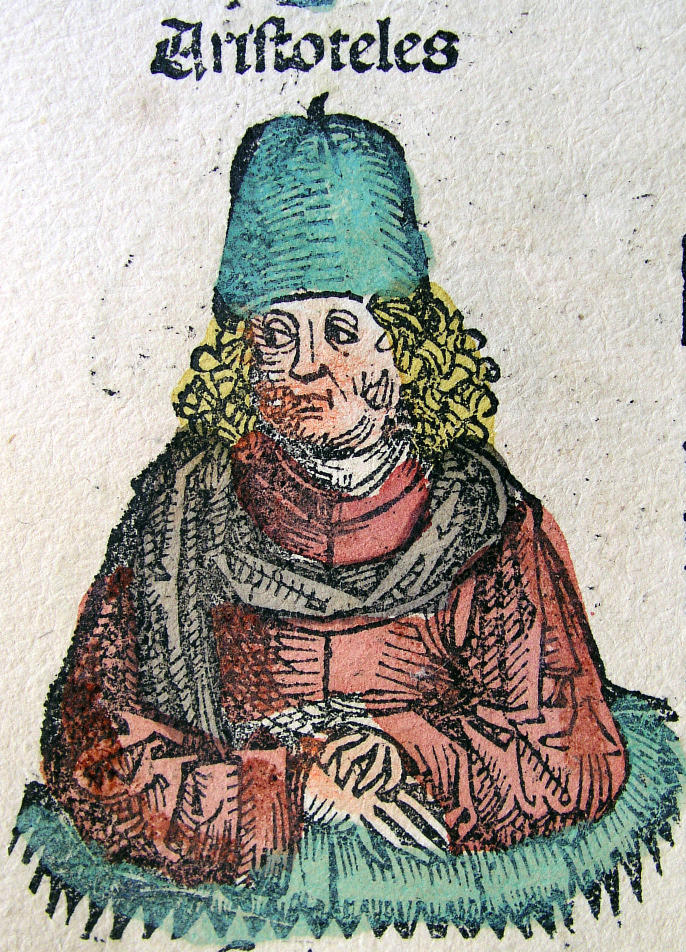
\includegraphics[width=0.3\textwidth]{Aristotle.jpg}
\end{center}
\caption{Аристотель глазами составителей Нюрнбергской хроники,
  1493}\label{fig:aristotle}
\end{figure}

Добавим лишь, что Аристотель в Нюрнбергской хронике
(см. Рис.~\ref{fig:aristotle}) был изображён в цвете, но в XXI веке
твёрдые копии сборников большинства конференций этим похвастаться не
могут. Поэтому в отношении всех цветных иллюстраций очень желательно
удостовериться в том, что и в чёрно-белом виде они не потеряют смысла.

\subsection{Прочие врезки и ссылки (заголовок II уровня)}

При врезке графиков и диаграмм следует придерживаться тех же правил,
что и при врезке изображений. Отдельно настоятельно рекомендуется
графики и диаграммы врезать, используя векторные форматы изображений,
так как это, опять же, более предсказуемо выглядит в твёрдой копии.

При наборе формул просьба по возможности использовать встроенные
средства офисного пакета.

Фрагменты текстов программ следует вставлять при помощи пакета
\texttt{listing}:

\begin{lstlisting}[language=C]
int main()
{
    return 0;
}
\end{lstlisting}

Библиографические ссылки следует оформлять стандартными средствами
\texttt{\textbackslash{}cite} и
\texttt{\textbackslash{}bibitem}~\cite{medvedev2011}. BibTeX, BibLaTeX
и подобные средства хорошо работают в собственных руках на собственных
текстах, но, попав в чужие, делают сюрпризы.  Поэтому просьба либо их
не использовать, либо использовать так, чтобы организаторы конференции
об этом не знали.

\section{Доказательства}

$$\int_0^t g(x)dW(x)$$

\begin{equation}
f(v) = 4 \pi v^2 \left( \frac{m}{2 \pi T} \right)^{3/2} \exp \left[ - \frac{m v^2/2}{T} \right].
\label{eq:maxwell_dist}
\end{equation}

\begin{enumerate}
	\item Зная конкретный вид $f(v)$, численно табулируется функция распределения
	\begin{equation}
	F_i (v_i) = \int\limits_{- \infty}^{v_i} f(v') dv'.
	\end{equation}
	\item По данным таблицы значений $\left\{ F_i ; v_i  \right\}$, интерполируется функция  $F^{-1}(v) = v(F)$.
	\item В силу свойств функции распределения $F \in \left[0,1\right]$. Тогда, очевидно, необходимо задать случайную величину в диапазоне от 0 до 1, подставить в полученную функцию и получить желаемый результат (рисунок \ref{fig:He(T=273)}).
\end{enumerate}
\begin{figure}[h!]
	\centering
%%	\includegraphics[width=0.85\linewidth]{./fig/ch4/He(T=273)}
	\caption{Проверка процедуры задания случайной величины по распределению Максвелла для гелия при $T = 273 \text{ К}$}
	\label{fig:He(T=273)}
\end{figure}

Далее требуется найти вектор магнитной индукции $\vec{B}_k = \left\{ B^{\rho}_k; B_k^z \right\}$, причём необходимо учесть, что её модуль определяется согласно формуле  а направление согласно правилу правого винта:
%%\eqref{eq:calcBcyl},
\begin{eqnarray}
B^{\rho}_k &=& \frac{\mu_0 R_k'}{2} \frac{I_k \left( R_k' - \rho_n \right)}{\left( \left( R_k' - \rho_n \right)^2 + \left( z_k - z_n \right)^2 \right)^{3/2}}, \\ \nonumber \\ \nonumber \\

B^{z}_k &=& \frac{\mu_0 R_k'}{2} \frac{I_k \left( z_k - z_n \right)}{\left( \left( R_k' - \rho_n \right)^2 + \left( z_k - z_n \right)^2 \right)^{3/2}}.
\end{eqnarray}

\section{Заключение}

В документе были представлены основные стили текста и макросы, которые
могут быть использованы при форматировании тезисов конференции СПИСОК.
Собственные тезисы рекомендуется набирать в этом документе, заменяя
текст и заголовки на свои.

\makeatletter\renewcommand{\refname}{\intl@references}\makeatother
\begin{thebibliography}{8}

\bibitem{medvedev2011} Медведев О. Use case: отладка реализации RISC
  процессора для FPGA // % Материалы 2-й межвузовской научной
  конференции по проблемам информатики<<СПИСОК-2011>>. --- % 2011. ---
  С. 7--12.
  \href{http://spisok.math.spbu.ru/txt/SPISOK-2011.pdf}{http://spisok.math.spbu.ru/txt/SPISOK-2011.pdf}

\end{thebibliography}

\end{document}
